\chapter{Introduction}

A l'heure où le film "Intouchables" a réussi à rassembler plus de 15 millions de spectateurs en moins de 6 mois, offrant, à ceux-ci, la démonstration d'une très belle amitié entre deux individus aux statuts fonctionnels, socials et culturels différents, on est en droit de se poser la question de savoir pourquoi il est toujours aussi difficile en 2012 d'intégrer un emploi lorsqu'on se trouve dans une situation de handicap.\\

L'importance de la reprise du travail dans la qualité de vie des personnes en situation de handicap n'est plus à démontrer. Il n'en demeure pas moins que les candidats sont nombreux mais les élus à la reprise professionnelle après un accident ou une maladie le sont moins. \\

Malgré un dispositif législatif important, les résistances et les verrous sont encore importants. \\

A quelques années d'une entrée dans la vie professionnelle, en tant que futur cadre dans les métiers de l'informatique et contenus de l'importance qu'occupe cette branche pour les personnes handicapées, j'ai souhaité engager une réflexion non seulement sur les difficultés rencontrées mais aussi sur les possibles réponses à apporter, dans la vie quotidienne des personnes marquées par le drame de l'accident ou de la maladie, donc d'un handicap acquis.


\begin{figure}
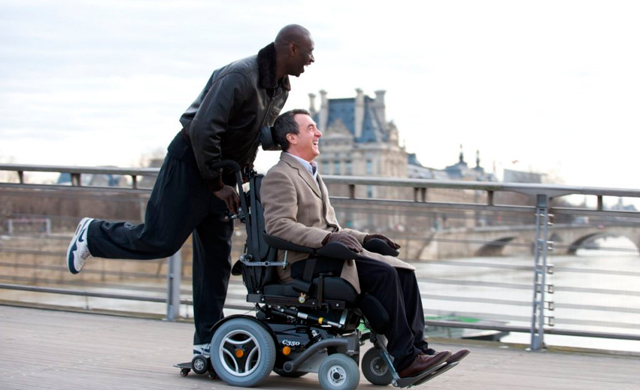
\includegraphics[scale=0.5]{figures/intouchable.jpg}
\centering
\end{figure}